\section{1º/2012}
\begin{exercicio}
  {1º/2012}{Arquiteturas de SO}
  {Admita um sistema operacional que é originalmente organizado segundo a estruturação microkernel no qual foi embutido um outro sistema operacional monolítico, por razões de desempenho. Como você classificaria esse sistema operacional? Por quê?}

\end{exercicio}

\begin{exercicio}
  {1º/2012}{Escalonamento de Processos}
  {Os escalonadores round-robin mantém, normalmente, uma fila de processos prontos, onde cada processo aparece uma só vez. Considere uma fila de prontos que mantém ponteiros para a tabela de processos. Qual seria o efeito de colocar dois ponteiros para o mesmo processo na fila de prontos $(A \rightarrow B \rightarrow C \rightarrow B)$?}

  O processo rodaria duas vezes por rodada, como se tivesse o dobro do quantum ou uma prioridade maior que os outros.
\end{exercicio}

\begin{exercicio}
  {1º/2012}{Escalonamento de Processos}
  {Considere o conjunto de $5$ processos e respectivos tempos de execução (quantum = $8 ms$). A ordem de chegada dos processos foi $A \rightarrow B \rightarrow C \rightarrow D \rightarrow E$ (do mais antigo para o mais recente). No momento de início de execução do algoritmo de escalonamento, todos os processos estão prontos. Diga a ordem na qual este conjunto será executado, considerando as políticas \textit{Round-Robin} e \textit{Shortest Job First (SJF)}.
  \begin{table}[H]
      \centering
      \begin{tabular}{cc}
        \hline \hline
        \textbf{Processo} & \textbf{Tempo de execução (ms)} \\ \hline
        A                 & 9                               \\
        B                 & 20                              \\
        C                 & 2                               \\
        D                 & 6                               \\
        E                 & 18                              \\
        \hline \hline
      \end{tabular}
    \end{table}
  }


    Estendemos a questão, inserindo também o resultado para política FCFS. Escrevemos em ordem, do primeiro para o último:

    \textbf{Round-robin:} $A \rightarrow B \rightarrow C \rightarrow D \rightarrow E \rightarrow A \rightarrow B \rightarrow E \rightarrow B \rightarrow E$

    \textbf{SJF:} $C \rightarrow D \rightarrow A \rightarrow E \rightarrow B$ (não tem \textit{quantum})

    \textbf{FCFS:} $A \rightarrow B \rightarrow C \rightarrow D \rightarrow E$ (não tem \textit{quantum})
\end{exercicio}

\begin{exercicio}
  {1º/2012}{Memória/Paginação}
  {Explique como funcionam as organizações, \textit{forward-mapped} (mapeamento direto) e tabela invertida, de páginas.}

  \textbf{Forward-mapped:} a tabela é indexada pelo endereço de página virtual, podendo existir uma entrada para cada endereço de página possível. A página indexa o \textit{frame} no qual ela deve residir na memória principal.

  \textbf{Tabela Invertida:} a tabela é indexada pelo \textit{frame}, segundo o espaço de endereçamento real. Para obter o índice correspondente da página virtual, é aplicada uma função \textit{hash}. Como é possível haver colisões, uma entrada pode conter uma lista de colisões, contendo as páginas que coincidiram naquele \textit{frame}.
\end{exercicio}

\begin{exercicio}
  {1º/2012}{Memória/Paginação}
  {Considere um sistema com espaço de endereçamento de $32$ bits, páginas de $4$ KBytes e espaço de endereçamento real de $26$ bits.
  \begin{enumerate}[label=(\alph*)]
    \item Quantas entradas são necessárias em uma tabela de páginas forward-mapped?
    \item E na tabela de páginas invertida?
  \end{enumerate}}

  Sabendo que o tamanho da página $P = 4KB = 4096B = 2^{12}$, temos:
  \begin{enumerate}[label=(\alph*)]
    \item \textbf{Forward-mapping:}
    $\frac{\text{espaço de endereçamento virtual}}{\text{/tamanho da paǵina}} =
    \frac{2^{32}}{2^{12}} = 2^{20}$;

    \item \textbf{Tabela Invertida:} $\frac{\text{endereçamento da memória}}{\text{tamanho da paǵina}} = \frac{2^{26}}{2^{12}} = 2^{14}$.
  \end{enumerate}
\end{exercicio}

\begin{exercicio}
  {1º/2012}{Drivers}
  {O que é uma controladora? Qual entidade do SO interage com ela?}

  A controladora é a parte eletrônica das unidades de entrada e saída (\textit{firmware}). Ela interage constantemente com os \textit{drivers} de dispositivo, recebendo comandos específicos de \textit{hardware} em seus registradores.
\end{exercicio}

\begin{exercicio}
  {1º/2012}{Sistemas de Arquivo}
  {Alguns sistemas de arquivo deletam todos os arquivos de usuário quando o usuário se desconecta da máquina (\textit{logoff}), a não ser que o usuário, explicitamente, diga quais arquivos devem ser permanentes. Comente esta abordagem em relação à abordagem tradicional.}

  Nela, temos:
  \begin{itemize}
    \item \textbf{Segurança}, pois os dados guardados serão descartados.
    \item \textbf{Desempenho}, pois ligará mais rápido já que não existe nenhuma associação a se fazer com os dados do usuário.
    \item \textbf{Economia}, podendo ser usada quando temos pouco espaço em disco.
  \end{itemize}
\end{exercicio}

\begin{exercicio}
  {1º/2012}{Sistemas de Arquivo}
  {Sobre \textit{buffer cache}:
  \begin{enumerate}[label=(\alph*)]
    \item Explique como as leituras e escritas em arquivos convencionais funcionam quando existe buffer cache.
    \item Explique como as leituras e escritas em arquivos convencionais funcionam quando não existe buffer cache.
  \end{enumerate}}

  \begin{enumerate}[label=(\alph*)]
    \item Quando uma operação de E/S é realizada, uma consulta a \textit{buffer cache} é realizada primeiro, onde o bloco solicitado é buscado em uma área de memória reservada. Caso não conste em memória, o bloco é buscado em disco, pelo controlador do disco, e colocado na \textit{buffer cache}, para completar a operação. Logo, as escritas não em disco não ocorrem no momento da operação, mas posteriormente. No caso de leituras, utiliza-se a leitura adiantada, ou seja, dados lidos adjacentes, que não fazem parte dos requisitados, são guardados na \textit{buffer cache}, seguindo o princípio da localidade.

    \item Neste caso, em todas as operações de E/S, o bloco é acessado diretamente do disco, resultando em um acesso mais lento. Logo, em uma leitura, o bloco é buscado em disco e, em uma escrita, o bloco é escrito no momento da requisição.
  \end{enumerate}
\end{exercicio}

\begin{exercicio}
  {1º/2012}{Deadlock/Produtor-Consumidor}
  {Apresente uma solução para o problema do produtor-consumidor utilizando unicamente locks.}
  \label{ex:prod-cons-locks}

  Antes, definimos:
  \begin{itemize}
    \item \texttt{MAX = } \textit{buffer size};
    \item \texttt{count = 0};
    \item Definimos o \textit{lock} \texttt{l} e inicializamos o mesmo.
  \end{itemize}

  \begin{figure*}[h]
    \begin{subfigure}{.45\textwidth}
      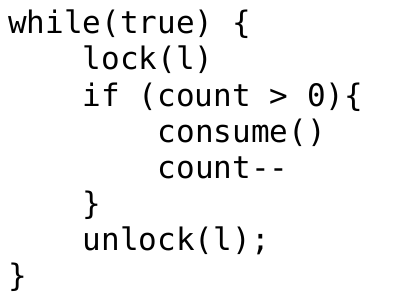
\includegraphics[width=\textwidth]{ex-lock-cons}
      \caption{Código Consumidor}
    \end{subfigure}
    ~
    \begin{subfigure}{.45\textwidth}
      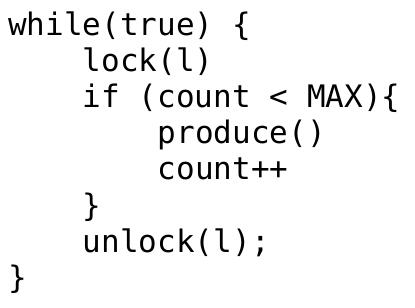
\includegraphics[width=\textwidth]{ex-lock-prod}
      \caption{Código Produtor}
    \end{subfigure}
  \end{figure*}
\end{exercicio}

\begin{exercicio}
  {1º/2012}{Processos/Escalonamento}
  {O algoritmo de escalonamento de processos FCFS pode ser considerado um caso particular do algortimo Round-Robin. Qual é esse caso?}

  Quando o quantum é infinito (teoricamente). Na prática, utiliza-se o \textit{quantum} como FFFF FFFF em arquiteturas de $32$ bits e FFFF FFFF FFFF FFFF em arquiteturas de $64$ bits.
\end{exercicio}

\begin{exercicio}
  {1º/2012}{Memória/Paginação}
  {Considere a seguinte sequência de referências à páginas:
  1,2,3,4,2,1,5,6,2,1,2,3,7,6,3,2,1,2,3,6. \newline
  Quantos page faults ocorrerão para os algoritmos FCFS, ótimo e LRU, supondo que a memória real possui $4$ frames? Considere que inicialmente a memória está vazia.}

  \textbf{Nota:} use como referência a estruturação do exercício da página \pageref{ex:pagination-1}. Aqui só inserimos a tabela de Ordem de Saída.

  \textbf{FCFS:} 14 \textit{page faults} \\
  \[
  \begin{array}{cccccccccccccccccccc}
1 & 2 & 3 & 4 & 2 & 1 & 5 & 6 & 2 & 1 & 2 & 3 & 7 & 6 & 3 & 2 & 1 & 2 & 3 & 6 \\ \hline
P & P & P & P & - & - & P & P & P & P & - & P & P & P & - & P & P & - & P & - \\
\\
1 & 2 & 3 & 4 & 4 & 4 & 5 & 6 & 2 & 1 & 1 & 3 & 7 & 6 & 6 & 2 & 1 & 1 & 3 & 3 \\
- & 1 & 2 & 3 & 3 & 3 & 4 & 5 & 6 & 2 & 2 & 1 & 3 & 7 & 7 & 6 & 2 & 2 & 1 & 1 \\
- & - & 1 & 2 & 2 & 2 & 3 & 4 & 5 & 6 & 6 & 2 & 1 & 3 & 3 & 7 & 6 & 6 & 2 & 2 \\
- & - & - & 1 & 1 & 1 & 2 & 3 & 4 & 5 & 5 & 6 & 2 & 1 & 1 & 3 & 7 & 7 & 6 & 6 \\
  \end{array}
  \]

  \textbf{Ótimo:} 8 \textit{page faults}. A idéia é sempre retirar a página a ser referenciada no futuro mais distante. \\
  \[
  \begin{array}{cccccccccccccccccccc}
1 & 2 & 3 & 4 & 2 & 1 & 5 & 6 & 2 & 1 & 2 & 3 & 7 & 6 & 3 & 2 & 1 & 2 & 3 & 6 \\ \hline
P & P & P & P & - & - & P & P & - & - & - & - & P & - & - & - & P & - & - & - \\
\\
1 & 2 & 2 & 2 & 1 & 2 & 2 & 2 & 1 & 2 & 3 & 6 & 6 & 3 & 2 & 2 & 2 & 3 & 6 & 1 \\
- & 1 & 1 & 1 & 2 & 1 & 1 & 1 & 2 & 3 & 6 & 3 & 3 & 2 & 3 & 3 & 3 & 6 & 1 & 2 \\
- & - & 3 & 3 & 3 & 3 & 3 & 3 & 3 & 6 & 2 & 2 & 2 & 6 & 6 & 6 & 6 & 1 & 2 & 3 \\
- & - & - & 4 & 4 & 4 & 5 & 6 & 6 & 1 & 1 & 1 & 7 & 7 & 7 & 7 & 1 & 2 & 3 & 6 \\
  \end{array}
  \]

  \textbf{LRU:} 10 \textit{page faults} \\
  \[
  \begin{array}{cccccccccccccccccccc}
1 & 2 & 3 & 4 & 2 & 1 & 5 & 6 & 2 & 1 & 2 & 3 & 7 & 6 & 3 & 2 & 1 & 2 & 3 & 6 \\ \hline
P & P & P & P & - & - & P & P & - & - & - & P & P & P & - & - & P & - & - & - \\
\\
1 & 2 & 3 & 4 & 2 & 1 & 5 & 6 & 2 & 1 & 2 & 3 & 7 & 6 & 3 & 2 & 1 & 2 & 3 & 6 \\
- & 1 & 2 & 3 & 4 & 2 & 1 & 5 & 6 & 2 & 1 & 2 & 3 & 7 & 6 & 3 & 2 & 1 & 2 & 3 \\
- & - & 1 & 2 & 3 & 4 & 2 & 1 & 5 & 6 & 6 & 1 & 2 & 3 & 7 & 6 & 3 & 3 & 1 & 2 \\
- & - & - & 1 & 1 & 3 & 4 & 2 & 1 & 5 & 5 & 6 & 1 & 2 & 2 & 7 & 6 & 6 & 6 & 1 \\
  \end{array}
  \]

\end{exercicio}

\begin{exercicio}
  {1º/2012}{Virtualização}
  {Os conceitos de \textit{full virtualization} e para \textit{virtualization} são explicados abaixo:
  \begin{itemize}
    \item \textit{Full Virtualization}: oferece uma abstração de máquina virtual que é uma cópia exata do hardware e, portanto, permite hospedar sistemas operacionais inalterados;
    \item \textit{Para Virtualization}: oferece uma abstração de máquina virtual que é similar, porém, não idêntica ao hardware e, por isso, requer que algumas modificações sejam feitas no sistema operacional hospedado.
  \end{itemize}
  Sabendo disso, qual estrutura de sistema operacional suporta \textit{full virtualization} e qual suporta para \textit{virtualization}? Justifique sua resposta.}

  \textbf{\textit{Full Virtualization}:} aceita qualquer organização do SO, pois contém todo o hardware.

  \textbf{\textit{Para Virtualization}:} não aceita monolítico ou camadas, pois eles possuem um maior acoplamento, por outro lado \textit{microkernel} e \textit{exokernel} podem ser modularizados e adicionados apenas os módulos necessários (existentes na máquina).
\end{exercicio}

\begin{exercicio}
  {1º/2012}{Organização de Sistemas Operacionais}
  {Complete o quadro abaixo com os valores (A - Alto, M - Médio, B - Baixo). Justifque sua resposta. Atenção: Cada linha deve conter os valores Alto, Médio e Baixo.
  \begin{table}[H]
    \centering
    \begin{tabular}{rcccc}
      \hline \hline
      \multicolumn{1}{l}{}             & \multicolumn{1}{c}{\textbf{Monolítico}} & \multicolumn{1}{c}{\textbf{Camadas}} & \multicolumn{1}{c}{\textbf{Microkernel}} & \multicolumn{1}{c}{\textbf{Exokernel}} \\ \hline
      \textbf{Visão Global do Sistema} & A & A & M & B \\
      \textbf{Extensibilidade} & B & B & M & A \\
      \textbf{Flexibilidade} & B & B & M & A \\
      \textbf{Manutenibilidade}& B & M & A & A\\
      \hline \hline
    \end{tabular}
  \end{table}}

  \textbf{Monolítico:}
  \begin{itemize}
    \item \textit{Visão Global do Sistema:} todas as funcionalidades do SO estão no kernel;
    \item \textit{Extensibilidade:} %%%%%%%%%%%%%%%TO DO%
    \item \textit{Flexibilidade:} pouca de estruturação torna o código custoso ao editar ou adicionar funcionalidade;
    \item \textit{Manutenibilidade:} é necessário uma atenção para não interferir em outras funcionalidades e toda alteração implica em recompilar todo o kernel;
  \end{itemize}

  \textbf{\textit{Camadas}:}
  \begin{itemize}
    \item \textit{Visão Global do Sistema:} todas as funcionalidades do SO estão no kernel;
    \item \textit{Extensibilidade:} %%%%%%%%%%%%%%%TO DO%
    \item \textit{Flexibilidade:}  %%%%%%%%%%%%%%%TO DO%
    \item \textit{Manutenibilidade:} apesar das camadas terem regras bem definidas, toda alteração implica em recompilar todo o kernel;
  \end{itemize}

  \textbf{\textit{Microkernel}:}
  \begin{itemize}
    \item \textit{Visão Global do Sistema:} alguns módulos estão no modo usuário, como gerência de memória e sistema de arquivos. Porém, ele possui visão global da gerência de processos e da memória dependente do hardware;
    \item \textit{Extensibilidade:} é possível adicionar mais módulos em modo usuário desde que estes respeitem o protocolo IPC;
    \item \textit{Flexibilidade:} diferentes estratégias de diferentes implementadas por servidores podem coexistir fora do kernel, exceto funcionalidades essenciais como gerência de processos e gerência de memória dependente do hardware;
    \item \textit{Manutenibilidade:} cada módulo é bem definido e pode ser tratado individualmente sem prejudicar os outros módulos;
  \end{itemize}

  \textbf{\textit{Exokernel}:}
  \begin{itemize}
    \item \textit{Visão Global do Sistema:} não conhece nenhuma abstração do SO, como gerência de processos ou sistema de arquivos. Apenas expõe o hardware e os protege;
    \item \textit{Extensibilidade:} é possível descarregar código no kernel, aumentando suas funcionalidades;
    \item \textit{Flexibilidade:} é possível executar diferentes LibOS em um mesmo exokernel, dando liberdade à aplicação de escolher qual LibOS ele executará no momento;
    \item \textit{Manutenibilidade:} além da facilidade de manipular bibliotecas que compõe abstrações da LibOS, caso alguma LibOS não esteja respondendo de modo adequado, é possível retirá-la de memória sem prejudicar os outros componentes e as outras LibOS em execução;
  \end{itemize}
\end{exercicio}
